\section{Einleitung} % (fold)
\label{sec:introduktion}

	\begin{figure}[b]
		% \center
		\begin{subfigure}[t]{0.33\textwidth}
			\center
			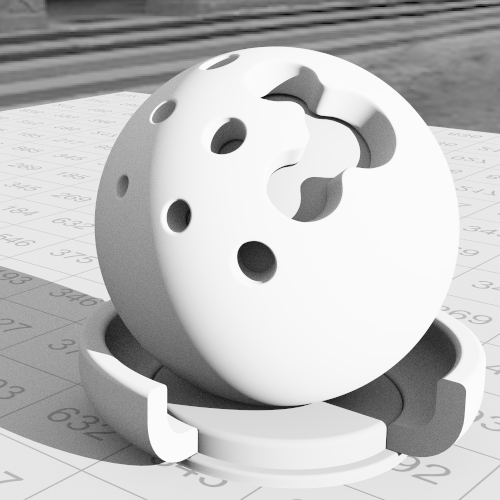
\includegraphics[width=0.95\textwidth]{pic/intro-shaderball-pt-1024-2.png}
			\caption{\parbox[t]{0.5\textwidth}{Path Tracing}}
		\end{subfigure}
		\begin{subfigure}[t]{0.33\textwidth}
			\center
			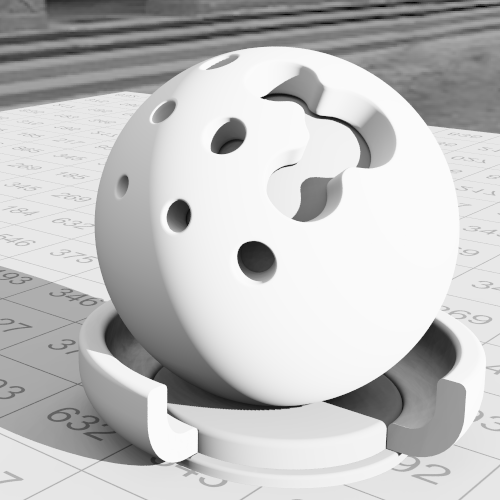
\includegraphics[width=0.95\textwidth]{pic/intro-shaderball-lightmap-462-2.png}
			\caption{\parbox[t]{0.5\textwidth}{Irradiance Map \\ Größe: $\sim462\unit{MiB}$}}
			\label{subfig:intro-shaderball-lm-big}
		\end{subfigure}
		\begin{subfigure}[t]{0.33\textwidth}
			\center
			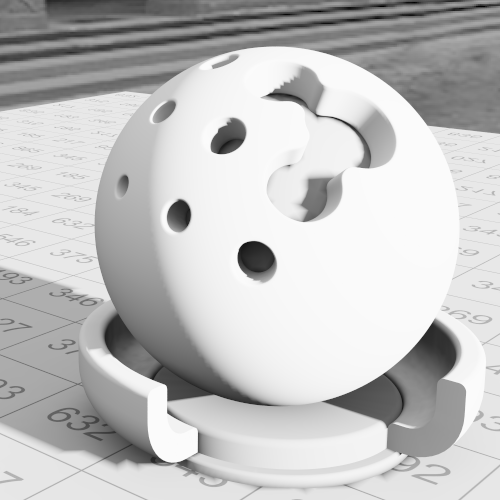
\includegraphics[width=0.95\textwidth]{pic/intro-shaderball-lightmap-2-2.png}
			\caption{\parbox[t]{0.5\textwidth}{Irradiance Map \\ Größe: $\sim2\unit{MiB}$}}
			\label{subfig:intro-shaderball-lm-small}
		\end{subfigure}
		\caption[Einfache Irradiance Maps der \enquote{Shaderball}-Szene mit \enquote{Uffizi Gallery}-HDR]{Die Bilder zeigen alle denselben Ausschnitt der \enquote{Shaderball}-Szene mit unterschiedlichen Shading-Verfahren. Die Lichtquellen bestehen aus einer direktionalen Lichtquelle und der \enquote{Uffizi Gallery}-HDR.}
		\label{fig:intro-shaderball}
	\end{figure}

	In der 3D-Computergrafik ist für die Erzeugung von realistischen Bildern die Simulation globaler Beleuchtungseffekte notwendig \cite{pbrt3}.
	Diese Lichteffekte ergeben sich formal als Lösung der \enquote{Rendergleichung} \cite{kajiya-lte}.
	Seit der Einführung dieser Gleichung im Jahre 1986 wurden verschiedene Algorithmen entwickelt, welche diese für beliebige Szenen numerisch lösen.
	Herauskristallisiert hat sich vor allem das \enquote{Path Tracing} \cite{pbrt3,kajiya-lte}.
	Dieses Verfahren kann die reale Beleuchtung beliebig genau und erwartungstreu schätzen.
	Aus diesem Grund werden die durch Path Tracing generierten Bilder meist als Referenzbild für die Bilder anderer Algorithmen verwendet, um deren Qualität zu untersuchen.

	Um nun verschiedene Materialien von Objekten simulieren zu können, werden häufig verschiedene Arten von Lichtstreuung an Oberflächen betrachtet.
	Eine der wichtigsten Arten ist gerade die ideale diffuse Streuung, welche der Szene ein grundlegendes plastisches Aussehen gibt.
	Sie ist unabhängig von der Richtung des einfallenden Lichtstrahls und damit auch invariant unter Änderung des Beobachtungspunktes \cite{intro-radiometry}.
	Für Path Tracing bedeutet dies, dass für jede Änderung der Kamera die eigentlich konstante Lichtverteilung neu berechnet werden muss.
	Diese Evaluierung nimmt aber auch den größten Rechenaufwand in Anspruch, da für jeden dieser Punkte Licht aus dessen gesamten Hemisphäre eingesammelt werden muss.
	Um also das Verfahren des Path Tracings zu optimieren, müssten die diffusen Lichtverhältnisse vorberechnet und auf der Oberfläche der Szene gespeichert werden \cite{irradiance-caching}.

	Besonders in der Computerspielindustrie wird dieses Problem mithilfe von sogenannten \enquote{Lightmaps} gelöst, welche für viele Punkte der Szene deren \enquote{Irradianz} in einer Textur speichern \cite{tricks-game}.
	Während des Renderings werden diese Werte dann zusammen mit der Farbe der Materialtextur ausgelesen, miteinander multipliziert und dargestellt.
	Die Generierung einer solchen Lightmap ist jedoch mit diversen Tücken verbunden, welche in vielen Fällen nur durch manuelle Optimierung beseitigt werden können.

	Aus diesem Grund führe ich im Laufe dieser Arbeit die sogenannten \enquote{Irradiance Maps} ein, die die Irradianz gegebener Punkte auf der Oberfläche der zugehörigen Szene speichern.
	Die benötigte Datenstruktur soll dabei speziell für die Verwendung von \enquote{Raytracing} und Path Tracing ausgelegt sein.
	Ich werde eine genauere Betrachtung der Irradianzbestimmung vornehmen, um so deren Prozess zu vereinfachen.
	Des Weiteren präsentiere ich einen Algorithmus zur adaptiven und automatischen Generierung einer solchen Irradiance Map.

	Abbildung \ref{fig:intro-shaderball} (Quelle aller Abbildungen: Markus Pawellek 2017) zeigt ein Beispiel, in welchem deutlich wird, dass Irradiance Maps in der Lage sind die diffusen Lichtverhältnisse sehr gut zu approximieren, jedoch bei schlechter Generierung viel Speicher benötigen (siehe \ref{subfig:intro-shaderball-lm-big}).
	Außerdem ist in \ref{subfig:intro-shaderball-lm-small} erkennbar, dass für einen Großteil der Szene eine vergleichsweise kleine Auflösung der Irradiance Map ausreicht.
	Es wird also auch darum gehen, diesen Sachverhalt bei der Konstruktion auszunutzen.

% section introduktion (end)